% Options for packages loaded elsewhere
\PassOptionsToPackage{unicode}{hyperref}
\PassOptionsToPackage{hyphens}{url}
\PassOptionsToPackage{dvipsnames,svgnames,x11names}{xcolor}
%
\documentclass[
  letterpaper,
  DIV=11,
  numbers=noendperiod]{scrartcl}

\usepackage{amsmath,amssymb}
\usepackage{iftex}
\ifPDFTeX
  \usepackage[T1]{fontenc}
  \usepackage[utf8]{inputenc}
  \usepackage{textcomp} % provide euro and other symbols
\else % if luatex or xetex
  \usepackage{unicode-math}
  \defaultfontfeatures{Scale=MatchLowercase}
  \defaultfontfeatures[\rmfamily]{Ligatures=TeX,Scale=1}
\fi
\usepackage{lmodern}
\ifPDFTeX\else  
    % xetex/luatex font selection
\fi
% Use upquote if available, for straight quotes in verbatim environments
\IfFileExists{upquote.sty}{\usepackage{upquote}}{}
\IfFileExists{microtype.sty}{% use microtype if available
  \usepackage[]{microtype}
  \UseMicrotypeSet[protrusion]{basicmath} % disable protrusion for tt fonts
}{}
\makeatletter
\@ifundefined{KOMAClassName}{% if non-KOMA class
  \IfFileExists{parskip.sty}{%
    \usepackage{parskip}
  }{% else
    \setlength{\parindent}{0pt}
    \setlength{\parskip}{6pt plus 2pt minus 1pt}}
}{% if KOMA class
  \KOMAoptions{parskip=half}}
\makeatother
\usepackage{xcolor}
\setlength{\emergencystretch}{3em} % prevent overfull lines
\setcounter{secnumdepth}{5}
% Make \paragraph and \subparagraph free-standing
\ifx\paragraph\undefined\else
  \let\oldparagraph\paragraph
  \renewcommand{\paragraph}[1]{\oldparagraph{#1}\mbox{}}
\fi
\ifx\subparagraph\undefined\else
  \let\oldsubparagraph\subparagraph
  \renewcommand{\subparagraph}[1]{\oldsubparagraph{#1}\mbox{}}
\fi


\providecommand{\tightlist}{%
  \setlength{\itemsep}{0pt}\setlength{\parskip}{0pt}}\usepackage{longtable,booktabs,array}
\usepackage{multirow}
\usepackage{calc} % for calculating minipage widths
% Correct order of tables after \paragraph or \subparagraph
\usepackage{etoolbox}
\makeatletter
\patchcmd\longtable{\par}{\if@noskipsec\mbox{}\fi\par}{}{}
\makeatother
% Allow footnotes in longtable head/foot
\IfFileExists{footnotehyper.sty}{\usepackage{footnotehyper}}{\usepackage{footnote}}
\makesavenoteenv{longtable}
\usepackage{graphicx}
\makeatletter
\def\maxwidth{\ifdim\Gin@nat@width>\linewidth\linewidth\else\Gin@nat@width\fi}
\def\maxheight{\ifdim\Gin@nat@height>\textheight\textheight\else\Gin@nat@height\fi}
\makeatother
% Scale images if necessary, so that they will not overflow the page
% margins by default, and it is still possible to overwrite the defaults
% using explicit options in \includegraphics[width, height, ...]{}
\setkeys{Gin}{width=\maxwidth,height=\maxheight,keepaspectratio}
% Set default figure placement to htbp
\makeatletter
\def\fps@figure{htbp}
\makeatother
% definitions for citeproc citations
\NewDocumentCommand\citeproctext{}{}
\NewDocumentCommand\citeproc{mm}{%
  \begingroup\def\citeproctext{#2}\cite{#1}\endgroup}
% avoid brackets around text for \cite:
\makeatletter
 \def\@biblabel#1{}
 \def\@cite#1#2{{#1\if@tempswa , #2\fi}}
\makeatother
\newlength{\cslhangindent}
\setlength{\cslhangindent}{1.5em}
\newlength{\csllabelwidth}
\setlength{\csllabelwidth}{3em}
\newlength{\cslentryspacing}
\setlength{\cslentryspacing}{0em}
\usepackage{enumitem}
\newlist{CSLReferences}{itemize}{1}
\setlist[CSLReferences]{label={},
  leftmargin=\cslhangindent,
  itemindent=-1\cslhangindent,
  parsep=\parskip,
  itemsep=\cslentryspacing}
\usepackage{calc}
\newcommand{\CSLBlock}[1]{#1\hfill\break}
\newcommand{\CSLLeftMargin}[1]{\parbox[t]{\csllabelwidth}{#1}}
\newcommand{\CSLRightInline}[1]{\parbox[t]{\linewidth - \csllabelwidth}{#1}\break}
\newcommand{\CSLIndent}[1]{\hspace{\cslhangindent}#1}

\KOMAoption{captions}{tableheading}
\makeatletter
\makeatother
\makeatletter
\makeatother
\makeatletter
\@ifpackageloaded{caption}{}{\usepackage{caption}}
\AtBeginDocument{%
\ifdefined\contentsname
  \renewcommand*\contentsname{Table of contents}
\else
  \newcommand\contentsname{Table of contents}
\fi
\ifdefined\listfigurename
  \renewcommand*\listfigurename{List of Figures}
\else
  \newcommand\listfigurename{List of Figures}
\fi
\ifdefined\listtablename
  \renewcommand*\listtablename{List of Tables}
\else
  \newcommand\listtablename{List of Tables}
\fi
\ifdefined\figurename
  \renewcommand*\figurename{Figure}
\else
  \newcommand\figurename{Figure}
\fi
\ifdefined\tablename
  \renewcommand*\tablename{Table}
\else
  \newcommand\tablename{Table}
\fi
}
\@ifpackageloaded{float}{}{\usepackage{float}}
\floatstyle{ruled}
\@ifundefined{c@chapter}{\newfloat{codelisting}{h}{lop}}{\newfloat{codelisting}{h}{lop}[chapter]}
\floatname{codelisting}{Listing}
\newcommand*\listoflistings{\listof{codelisting}{List of Listings}}
\usepackage{amsthm}
\theoremstyle{plain}
\newtheorem{lemma}{Lemma}[section]
\theoremstyle{definition}
\newtheorem{definition}{Definition}[section]
\theoremstyle{plain}
\newtheorem{theorem}{Theorem}[section]
\theoremstyle{definition}
\newtheorem{example}{Example}[section]
\theoremstyle{plain}
\newtheorem{proposition}{Proposition}[section]
\theoremstyle{remark}
\AtBeginDocument{\renewcommand*{\proofname}{Proof}}
\newtheorem*{remark}{Remark}
\newtheorem*{solution}{Solution}
\makeatother
\makeatletter
\@ifpackageloaded{caption}{}{\usepackage{caption}}
\@ifpackageloaded{subcaption}{}{\usepackage{subcaption}}
\makeatother
\makeatletter
\makeatother
\ifLuaTeX
  \usepackage{selnolig}  % disable illegal ligatures
\fi
\IfFileExists{bookmark.sty}{\usepackage{bookmark}}{\usepackage{hyperref}}
\IfFileExists{xurl.sty}{\usepackage{xurl}}{} % add URL line breaks if available
\urlstyle{same} % disable monospaced font for URLs
\hypersetup{
  pdftitle={Bridging Diffusion Geometry to Curvature},
  pdfauthor={Kincaid MacDonald; Dhananjay Bhaskar; Yanlei Zhang; Ian Adelstein; Smita Krishnaswamy},
  pdfkeywords={Manifold Learning, Geometric Deep Learning, Graph
Curvature, Point Clouds, Diffusion Geometry, Topological Data
Analysis, Neural Loss Landscapes, Single-Cell Data},
  colorlinks=true,
  linkcolor={blue},
  filecolor={Maroon},
  citecolor={Blue},
  urlcolor={Blue},
  pdfcreator={LaTeX via pandoc}}

\title{Bridging Diffusion Geometry to Curvature}
\author{Kincaid MacDonald \and Dhananjay Bhaskar \and Yanlei
Zhang \and Ian Adelstein \and Smita Krishnaswamy}
\date{2024-08-12}

\begin{document}
\maketitle
\begin{abstract}
Modeling data geometry has proven a rich source of interpretable
features: quantifying `the shape' of molecules, cellular trajectories,
and code enhances downstream classification performance. Yet, creating
these features requires a theoretical `Rosetta Stone' to bridge
geometric theory into the noisy, discrete world of real data. Various
bridging paradigms have been proposed, most prominently \emph{diffusion
geometry} -- and have given rise to manifold distance estimators, and
manifold embedding techniques.However, the estimation of curvature
remains relatively unexplored. Curvature, being the most local geometric
measure, is among the most challenging concepts to bridge into the
discrete realm; for this reason, it is also a sterling test a given
paradigm's ability to translate geometric theory into the sampled
data.Here, we introduce \emph{Diffusion Curvature}, a new definition of
scalar curvature on point clouds which inherits diffusion geometry's
robustness to noise and sampling. In our benchmarks, diffusion curvature
proves itself the \emph{only} method capable of robustly differentiating
positive and negative curvature in high dimensions, while its absence of
parameters requiring user tuning makes it significantly more
user-friendly than other methods.We describe theoretical connections
between diffusion curvature and the Ollivier-Ricci curvature, and
introduce a general paradigm for comparing diffusions across graphs.We
apply diffusion curvature to neural loss landscapes, single-cell RNA
data {[}bit about what we find{]} motivating the practical utility of
our method.
\end{abstract}
\begin{center}\rule{0.5\linewidth}{0.5pt}\end{center}

\newcommand\Kaly[1]{\textcolor{blue}{Kaly: [[[#1]]]}}

\section{Introduction}\label{introduction}

The \emph{Manifold Assumption} is among machine learning's most prolific
muses. Given only the knowledge that the local Euclidean distances
between raw datapoints are meaningful, the Assumption grants a fount of
theoretical intuition and methodological inspiration. It lies behind
low-dimensional embedding and visualization techniques like PHATE,
manifold distance estimators like HeatGeo, and the entire field of
Topological Data Analysis (Moon et al. 2019; Huguet et al. 2023). It
also invites one to use that theoretical inspiration to design new
practical methods. Doing so, however, requires facing a sort of troll:
one must bridge the idealized, analytic spaces of theory with the noisy,
discrete world of real data. This is easier in some parts of theory than
others. In particular, doing so is harder the more \emph{locally} one
tries to apply the Assumption. Global topological features are easier;
manifold distances, harder; and manifold \emph{curvatures}, perhaps the
hardest of all.

But while distances or topological descriptors are widely used and have
ready utility, one might be excused for asking ``why care about
curvatures?'' A response, becoming more coherent with a raft of new
graph and point-cloud curvature methods, is for its utility as a
hyper-local descriptor of manifold geometry. There are many techniques,
from Topological Data Analysis, to manifold distances estimators or
graph or manifold embedding techniques that give global features.
Curvature answers the opposing question: ``\emph{around this point, in
this neighborhood, what's happening to the local geometry}?'' Such
answers are directly interpretable in domains like single-cell biology,
where curvature can indicate the extent of cell differentiation. They
have also been shown to exceed and enhance the local discriminative
powers of Graph Neural Networks (cite Bastian, COMPASS). (ADD other
areas of application; reference Hickok \& Sritharan). loss landscapes,
eg

But notions of graph and point-cloud curvature are also particularly
poignant for their theoretical implications. On one level, they are
attempting to square an impossible circle. While global, topological
features have a theoretical tolerance for discrete data, Riemannian
geometry is built upon measures of \emph{infinitesimal} locality -- and
curvature is the most local of Riemannian measurements. This is
precisely where discrete data is the least reliable. Globally, point
clouds can be recognized as manifolds, but zoom in to the locale of
individual points, and the inevitable presence of noise and varying
densities imbues the discrete manifold with a Heisenberg-like
uncertainty: the smaller you go, the less you know of the local
structure.

Hence the need for that `bridge' -- a Rosetta Stone, if you will --
between the continuous, analytically-specified spaces of theory and the
messy realities of actual data. The several existing discrete curvature
methods chiefly use one of two classes of bridge: optimal transport, as
in the field's bulwark, Ollivier-Ricci curvature, and tangent-plane
approximation, as used by methods like Sritharan and Adal-PCA (REFINE).
This choice may seem inconsequential -- it's only curvature, after all
-- but precisely because curvature is so local, the ability of such a
bridge to estimate curvature qualifies it for a much broader role: as a
means to bring \emph{general} geometric ideas into the discrete realm.

How effective are these bridges? To explore this, we develop a
comprehensive benchmarking suite, and present the first quantitative
comparison of discrete curvature methods -- probing their tolerance to
noise, high dimensions, and parameter perturbations. The landscape is,
unfortunately, rather dismal. Most existing methods reliably fail to
distinguish between negative and positive curvatures in high dimensions,
degrade under small quantities of noise, and are highly dependent on the
user tuning parameters which the user -- not having access to the
ground-truth curvatures -- has no ability to tune. Graph curvature
methods like Ollivier-Ricci and Forman-Ricci are difficult to translate
to higher-density point cloud data, and point cloud methods like
Sritharan, Hickok, and Adal-PCA depend on higher-order geometric
concepts (like volumes and distances) whose estimation depends on
curvature. This is both discouraging to those practitioners and
academics thinking of incorporate curvature estimation in their
research, and suggestive of a larger cavity in geometric featurization.
None of these existing bridges pass the curvature test.

Perhaps the most well-traveled bridge in other areas of geometric
estimation is data diffusion, or as often styled, ``Diffusion
Geometry''. Beginning in 2006 with Coifman \& Lafon's ``Diffusion maps''
(Coifman and Lafon 2006), this bridge operates through repeated
application of a \emph{diffusion operator} which can be thought of
either as simulating heat diffusion, or performing a weighted random
walk across data points. When iterated, this diffusion process performs
a sort of `integration' of local structure into a set of semi-local
features which enable one to escape the confounding factors noise and
sparsity. This idea underlies distance estimators like Diffusion
Distances and HeatGeo Huguet et al. (2023), dimensionality-reduction
methods like PHATE and GAGA (Moon et al. 2019), and even a deep-learning
based inference of the local Riemannian metric (Fasina et al. 2023).
More generally, the diffusion-based \emph{graph scattering transform}
has inspired new graph neural network architectures with
state-of-the-art performance on baselines requiring fine-grained local
discrimination. (CHECK. IS THIS TRUE?)

Can this bridge of diffusion geometry pass the `curvature test'?
Moreover, can it produce a curvature method robust enough to noise,
dimension, and parameterization to be practically useful on point cloud
data? In Bhaskar et al. (2022), we gave a preliminary positive answer
with \emph{diffusion laziness curvature}, an unsigned curvature derived
from the diffusion operator. This strongly suggested that the powered
diffusion operator contains curvature information, but was lacking both
in theoretical pedigree and experimental validation on anything beyond
2-dimensional manifolds. We now present the maturation of this work.

\emph{Diffusion Curvature} is a signed curvature based on diffusion
geometry. It is resilient to noise, requires no user-tuned parameters,
and robustly distinguishes between signs in high dimensions and under
noise. We prove theoretical connections between diffusion curvature and
the field's bulwark, \emph{Ollivier-Ricci Curvature}, which position
diffusion curvature as a point-wise adaptation of Ollivier-Ricci - and
further connect diffusion geometry to the optimal transport literature.
More broadly, the success of diffusion-based techniques in determining
curvature strongly motivates diffusion geometry as the missing Rosetta
Stone between geometric theory and data science practice.

\section{Background}\label{background}

\subsection{Curvature in the Continuous
Setting}\label{curvature-in-the-continuous-setting}

There are many definitions of curvature on Riemannian manifolds. In this
work, we focus on discrete analogs to the \emph{Ricci} curvature
\(\text{Ric}(x,y)\), which we'll briefly motivate in the continuous
setting.

Imagine two spheres of equal radius centered at \(x\) and \(y\) in a
Riemannian manifold \(\mathcal{M}\). Intuitively, the Ricci curvature
between \(x\) and \(y\) measures the difference between the distance of
these midpoints, and the average distance between corresponding points
in each sphere. In an area of positive Ricci curvature, points in
spheres are, on average, closer than their midpoints; in negative Ricci
curvature, the points in the sphere are further, on average, than the
midpoints. This is formally described by first defining the
\emph{sectional curvature} as the contraction of length incurred by
parallel transport through a 2-plane of the manifold, then defining the
Ricci curvature as an average of the sectional curvatures between two
points. For the present work, we needn't reproduce the full definitions,
but we will recall some properties of manifolds with Ricci curvature
bounded from below by some \(k\).

First, recall the relation between curvature and volume. In spaces of
high positive curvature, the volume of a ball is \emph{smaller} than a
ball of the same radius in a flat space, and even smaller than a ball of
the same radius in a hyperbolic space. This is formally expressed by the
Bishop Gromov inequality ({``Bishop--{Gromov} Inequality''} 2021).

\begin{theorem}[Bishop-Gromov]\protect\hypertarget{thm-bishop-gromov}{}\label{thm-bishop-gromov}

Let \(\mathcal{M}\) be a complete \(d\)-dimensional Riemannian manifold
with \(Ric(x,y) > (d - 1)k\) for all \(x,y \in \mathcal{M}\) and
\(k \in \mathbb{R}\). Let \(M_{K}^d\) be the complete \(d\)-dimensional
simply connected space of constant sectional curvature \(k\). Denote by
\(B(x,k)\) the ball of radius \(k\) centered at \(x\). Then for any
\(x \in \mathcal{M}\) and \(x_{k} \in M_{K}^d\), the function

\[
\phi(r) = \frac{\operatorname{Vol}B(x,r)}{\operatorname{Vol}B(x_{k},r)}
\] is non-increasing on \((0,\infty)\).

\end{theorem}

This phenomenon of diminishing volume in positive curvature is related
to the convergence of geodesic rays. In the plane (or saddle), two
geodesic rays extending from the same point in different directions will
never intersect. But on the sphere, they \emph{will} meet again -- at
the opposite pole. This convergence constrains the maximum diameter a
space of positive curvature may have, as expressed in the Bonnet-Myers
Theorem (Ollivier 2009):

\begin{theorem}[Bonnet-Myers]\protect\hypertarget{thm-bonnet-myers}{}\label{thm-bonnet-myers}

Let \(X\) be an \(d\)-dimensional Riemannian manifold. Let
\(\inf \operatorname{Ric}(X)\) be the infimum of the Ricci curvature
\(\operatorname{Ric}(v, v)\) over all unit tangent vectors \(v\). Let
\(S^d \subset \mathbb{R}^{d+1}\) be the unit sphere of the same
dimension as \(X\). Then, if
\(\inf \operatorname{Ric}(X) \geqslant \inf \operatorname{Ric}\left(S^d\right)\)
then \(\operatorname{diam} X \leqslant \operatorname{diam} S^d\).

\end{theorem}

We'll encounter versions of Bishop-Gromov and Bonnet-Myers in our
discrete setting. But first, let's describe the construction and
properties of our specific discrete setting.

\subsection{The Discrete Setting}\label{the-discrete-setting}

Within the ambient setting of points \(x_{i} \in \mathbb{R}^D\), the
Euclidean distances between the points in our point cloud are not very
useful. To perform geometric analysis, we want the manifold's
\emph{geodesic} distances between \(x_{i}, x_{j} \in \mathcal{M}\),.
However, manifolds are locally euclidean, so within a sufficiently small
neighborhood of \(x_{i} \in \mathcal{M}\) , the euclidean distances are
accurate. This is the basis of graph construction: retain only the
trustworthy local distances, discard the rest, and then ``integrate''
over the local neighborhoods to recover features of the global geometry.

A graph \(G = (V, E)\) is a collection of \(n\) vertices \(v_{i} \in V\)
connected by (possibly weighted) edges \(e_{ij} \in E\) . It is
efficiently represented by a single \emph{adjacency} (or
\emph{affinity}) matrix \(A \in \mathbb{R}^{n \times n}\), where
\(A_{ij}\) expresses the degree of connection between the vertices
\(v_{i}\) and \(v_{j}\). In a binary adjacency matrix, \(A_{ij}=1\) iff
there is an edge between \(v_{i}\) and \(v_{j}\). In a weighted affinity
matrix, \(0<A_{ij}<1\) with a higher affinity indicating a closer
connection between the nodes.

One can construct an affinity matrix from a point cloud with the
following algorithm: 1. Compute the matrix \(D\) of pairwise euclidean
distances between points, so that \(D_{ij}=\|x_{i}-x_{j}\|_{2}\). 2.
Apply a kernel \(\kappa\) to the distances to construct the affinity
matrix, where \(A_{ij} = \kappa(D_{ij})\). This is typically the
gaussian kernel: \[
\kappa(y) = \frac{1}{\sqrt{ 2\pi }\sigma}\exp\left( -\frac{y}{\sigma^2} \right)
\] There are a variety of heuristics for selecting an appropriate kernel
bandwidth \(\sigma\). In this paper, we use an adaptive kernel
bandwidth, in which, when computing \(k(D_{ij})\), \(\sigma\) is set to
the mean distance from the points \(x_{i}\) and \(x_{j}\) to their
\(k\)-th nearest neighbor.

After building our graph affinity matrix \(A\), we created a new
representation of the point cloud \(X\) -- turning it from an
\(n \times D\) matrix of unwieldy ambient coordinates into an
\(n \times n\) matrix of pairwise connections between points. The
challenge is now to reassemble this information of local connectivity to
recover the features of \(\mathcal{M}\). Graph diffusion does precisely
this.

\subsection{Graph Diffusion}\label{graph-diffusion}

By row-normalizing \(A\), one obtains the graph diffusion matrix
\(P = D^{-1}A\), which is a commonly-used method of ``integrating'' the
local connectivity of the graph \(A\) into global geometric descriptors
of \(\mathcal{M}\). Coifman and Lafon (Coifman and Lafon 2006) proved a
correspondence between iterated graph diffusion \(P^t\) and the Neumann
heat kernel on \(\mathcal{M}\). Their technique, \emph{Diffusion Maps},
uses the Euclidean distances between eigencoordinates of \(P\) to
approximate the geodesic distances on \(\mathcal{M}\). The visualization
technique \(PHATE\) (Moon et al. 2019) constructs a low-dimensional
embedding of a point cloud \(X\) such that a distance between the
transition probabilities \(P\) of \(X\) is preserved in the embedding.
(More on properties of phate, trajectory preservation.) \emph{Diffusion
Earth Mover's Distance} (A. Y. Tong et al. 2021) efficiently
approximates the transportation distance between distributions on a
graph using multi-scale wavelet transform obtained by applying different
scales of diffusion. \emph{LEGSNet}`s ``learnable geometric scattering''
computes tunable scales of diffusion with a graph neural network and
achieves state of the art performance on biochemistry graph
classification (A. Tong et al. 2021). These are but a few of the many
manifold learning techniques based in diffusion.

Constructing the diffusion matrix from the affinity matrix \(A\) is
straightforward: you simply row-normalize \(A\), with an optional step
to normalizing by density.

Here is the algorithm presented in Coifman and Lafon (Coifman and Lafon
2006):

\begin{enumerate}
\def\labelenumi{\arabic{enumi}.}
\tightlist
\item
  (Optional) Compute an \emph{anisotropic density normalization} on
  \(A\), obtaining the anisotropic adjacency matrix \(A_{\star}\).
\item
  Construct the degree matrix \(D\), whose diagonal entries are the
  rowsums of \(A\), i.e.~\(D_{ii} = \sum_{j}A_{ij}\).. The other entries
  are zeros.
\item
  Define \(P = D^{-1} A\), the graph diffusion matrix.
\end{enumerate}

\begin{itemize}
\tightlist
\item[$\square$]
  Clean this up: get anisotropic equation, and clarify the role of the
  self affinity. When is it removed? When is laziness added?
\end{itemize}

\(P\) has several nice properties. The rows \(P[i]\) give the transition
probabilities of a single step random walk starting at point \(x_{i}\);
each row \(P[i]\) can be viewed as a probability distribution centered
at \(x_{i}\). This is preserved under powers of the matrix. The rows of
\(P^t\) still sum to 1, and \(P^t[i]\) now gives the probability
distribution of a \(t\)-step random walk starting at \(x_{i}\).

Although \(P\) is not symmetric, it is conjugate to a symmetric matrix,
via \(D^{0.5}PD^{-0.5} = D^{-0.5}AD^{-0.5}\), granting it a full basis
of real-valued eigenvectors and eigenvalues. These eigenvectors are
shared with the normalized graph Laplacian
\(L = I - D^{-0.5}AD^{-0.5}\). The eigenvalues of \(P\) have magnitude
less than or equal to 1. Powering the matrix \(P^t\) thus corresponds to
powering the eigenvalues \(\lambda_{i}^t\) of \(P\), via diagonalization
\[
P^t = \Psi \Lambda^t \Psi^T
\] This is similar to applying a low-pass filter to the graph. As \(t\)
increases, the smallest eigenvalues decay fastest under repeated
powering, and their corresponding eigenvector vanishes from the
eigenbasis -- leaving only the largest \(\lambda_{i}\), whose
eigenvectors trace global geometric features.

This is a remarkable feature of the diffusion matrix: the ability to
``denoise'' itself by iterating the random walk over larger time scales.
Intuitively, the paths through the data most robustly trafficked by
random walkers are those supported by multiple high-probability
connections from independent starting points.

\subsection{Ollivier-Ricci Curvature}\label{ollivier-ricci-curvature}

Developed by Yann Ollivier in 2007, \emph{Coarse Ricci Curvature} (or
sometimes, ``Ollivier Ricci Curvature'') is a direct translation of
Ricci curvature to discrete metric spaces like graphs (Ollivier 2009).
Several classical properties of Ricci curvature can be extended to the
graph setting using Coarse Ricci Curvature. Ollivier has, for instance,
proven versions of concentration inequalities, Bonnet Myers (more).
Coarse Ricci Curvature has, in this way, become something of a bridge
between continuous and coarse geometry. The basis of this bridge is
optimal transport, and specifically, the 1-Wasserstein distance.

In the Riemannian setting, Ricci curvature captures the phenomenon that,
in positive curvature, ``small spheres are closer (in transportation
distance) than their centers are'' (Ollivier 2009). On the sphere, for
instance, imagine two circles centered on the north and south poles:
every point in each circle is closer to the corresponding point in the
opposite circle than are the circles' centers. This effect diminishes as
one moves the circles closer together, but never reaches equality. In
negatively curved spaces, the discrepancy reverses, while in a flat
space, the average distance between the points of the circles is the
distance between the centers.

Coarse Ricci Curvature captures a similar phenomenon on graphs. Instead
of spheres, it uses locally-centered probability distributions defined
by random walks. And to measure the distance between these walks, it
uses the 1-Wasserstein (or Earth Mover's) distance. We'll briefly define
each.

The 1-Wasserstein distance is a measure of the distance between
probability distributions. Given distributions \(\mu_{x}\) and
\(\mu_{y}\) over some shared space \(X\), the Wasserstein distance
quantifies the smallest amount of ``work'' needed to transform one
distribution into another, by transporting probability ``mass'' between
pairs of points over the ground metric \(d(x,y)\):

\begin{definition}[1-Wasserstein
Distance]\protect\hypertarget{def-1-wasserstein}{}\label{def-1-wasserstein}

The 1-Wasserstein distance between distributions \(\mu_{x}\) and
\(\mu_{y}\) is
\[ W_{1}(\mu_{x},\mu_{y}) := \inf_{\xi \in \Pi(\mu_{x},\mu_{u})} \int \int d(x,y) \, d\xi(x,y) \]
where the ``transportation plan'' \(\xi\) is drawn from the space
\(\Pi(\mu_{x},\mu_{y})\) of joint probability distributions over
\(X \times X\) which project onto \(\mu_{x}\) and \(\mu_{y}\). In the
discrete setting, this translates naturally into an infimum over a
summation.
\[W_{1}(\mu_{x},\mu_{y}) := \inf_{\xi \in \Pi(\mu_{x},\mu_{y})} \sum_{x \in X} \sum_{y \in X} d(x,y) \xi(x,y)\]

\end{definition}

What is the analog on a graph of a ``small sphere'' around a point?
Ollivier replaces spheres with a family of measures \(m_{x}(\cdot)\)
defined for each point \(x\), where

\begin{enumerate}
\def\labelenumi{\arabic{enumi}.}
\tightlist
\item
  Each \(\mu_{x}(\cdot)\) depends measurably on \(x\), i.e.~the map
  \(x \to \mu_{x}\) is measurable.
\item
  Each \(\mu_{x}(\cdot)\) has finite first moment, or \emph{Jump},
  i.e.~for some \(o \in X\) \(\int d(o,y) \mu_{x}(y) \, dx < \infty\).
\end{enumerate}

In graphs, Ollivier defines these \(\mu_x\) as the probability
distributions created by a single-step random walk from the point \(x\).

With a transition probability \(\alpha\), and equal probability of
moving to each of \(x\)'s neighbors on the graph,
\(\mu_{x}(x) = (1-\alpha)\) and \(m_{x}(y) = \alpha\) if \(y \in N(x)\)
or \(0\) otherwise.

This is analogous to defining \(m_{x} = P e_{x}\), if \(P\) is the
diffusion matrix created from a binary adjacency matrix. Note, however,
that there is nothing limiting us to binary adjacency matrices, or even
single steps of diffusion; the two conditions above are equally
satisfied by weighted adjacency matrices and \(t\)-step diffusions, and
in sparse or noisy graphs, this may be desirable.

\begin{definition}[Coarse Ricci
Curvature]\protect\hypertarget{def-coarse-ricci-curvature}{}\label{def-coarse-ricci-curvature}

The \emph{Coarse Ricci Curvature} between \(x\) and \(y\) is
\[\kappa(x, y):=1-\frac{W_1\left(m_x, m_y\right)}{d(x, y)}\]

\end{definition}

There are a number of provisos attached to this definition, which tries
to approximate a continuous phenomenon within discrete constraints.
These constraints, and the relationship between Ricci and Ollivier's
coarse Ricci curvature are illustrated Ollivier's Example 2.6 (Ollivier
2009):

\begin{example}[]\protect\hypertarget{exm-ollivier-example-2.6}{}\label{exm-ollivier-example-2.6}

Let \((X,d)\) be a smooth Riemannian manifold of dimension \(d\) and let
\(\text{vol}\) be the Riemannian volume measure. Let \(\epsilon>0\)
small enough and consider the ball of radius \(\epsilon\) around each
point \(x\). Let \(x,y \in X\) be two sufficiently close points. Let
\(v\) be the unit tangent vector at \(x\) directed towards \(y\). The
coarse Ricci curvature along \(v\) is then
\[\kappa(x,y) = \frac{\epsilon^2 \text{Ric}(v,v)}{2(d+2)}+o(\epsilon^3 + \epsilon^2d(x,y))\]

\end{example}

Hence the coarse Ricci curvature applied to a manifold recovers the
Ricci curvature, up to a scaling factor contingent on dimension, and
plus an error term that grows with the radius of ball and distance
between points.

Ollivier's choice not to scale \(\kappa(x,y)\) by dimension is
interesting, and likely motivated by his application of coarse Ricci
curvature to graph-like spaces for which dimension isn't clearly
defined, like social networks. Within our domain of point-cloud data,
incorporating dimension may be desirable; without it, spaces of high
dimension can be conflated with spaces of lower dimension but higher
negative curvature.

A result on coarse Ricci curvature which will prove useful concerns the
\emph{contraction (or expansion) of measure} that occurs under diffusion
in spaces of positive (or negative) curvature. This is Ollivier (2009)'s
Proposition 20:

\begin{proposition}[\(W_1\) Contraction of
Measure]\protect\hypertarget{prp-ollivier-contraction-of-measure}{}\label{prp-ollivier-contraction-of-measure}

Let \((X,d,m)\) be a metric space with a random walk. Let
\(\kappa \in \mathbb{R}\). Then we have \(\kappa(x,y) \geq \kappa\) for
all \(x,y \in X\) iff for any two probability distributions
\(\mu, \mu' \in \mathcal{P}(X)\) one has

\[
W_{1}(\mu \star m, \mu' \star m) \leq (1-k)W_{1}(\mu, \mu')
\] Where \[
 \mu \star m := \int_{{x \in X}} d\mu(x)m_{x} \, dx
\]

\end{proposition}

\section{Methods}\label{methods}

We consider a measure space \((X,p)\) equipped with a random walk,
e.g.~a point cloud and a diffusion operator derived as above. In this
section, we define a new notion of curvature deriving from this random
walk.

The core intuition of Diffusion Curvature is that the \emph{laziness} of
random walks on a graph is a proxy for the curvature of the underlying
manifold. Picture a ``random walker'' drunkenly traversing a sphere. If
he manages, over the course of several steps, to wander to the opposite
pole, he has many ways of getting back to where he started. By contrast,
if he begins on the top of a (negatively-curved) saddle and wanders down
one side, any path aside from exactly retracing his steps incurs a steep
penalty in extra distance. On the sphere, the random walker is more
likely to find his way home: his walks are ``lazier''.

Our previous paper (Bhaskar et al. 2022) measured this laziness
directly, as the return probability within a k-neighborhood of the
starting point. This required tuning the parameter \(k\), and neglected
the information provided by probabilities outside of this neighborhood.

We refine our previous definition of diffusion laziness by replacing the
neighborhood-sum with a distributional distance measure \(D\) between a
dirac \(\delta_{x}\) and its \(t\)-step diffusion \(p_{x}^X(t)\). This
provides a more sensitive and parameter-free measure of how `spread out'
the diffusion is.

\begin{definition}[Diffusion
Energy]\protect\hypertarget{def-energy-of-diffusion}{}\label{def-energy-of-diffusion}

Given some distributional distance \(D\), the \(D\)-energy snapshot of a
diffusion \(p_{x}^X(t)\) at time \(t\) is \[
l_{X}(x,t) := D\left(\delta_x, p_x^X(t)\right)
\]

\end{definition}

By \(p_{x}^X(t)\), we indicate the \(t\)-step diffusion of the dirac
\(\delta_{x}\) centered at \(x \in X\), using the diffusion operator for
the measure space \(X\). We use the term `Diffusion Energy' in reference
to our previous work (CITE), which measured curvature via `Diffusion
Laziness'. That laziness measurement increased with positive curvature;
diffusion energy does the opposite, increasing with more negative
curvature.

The distributional distance \(D\) may be the Wasserstein-1 distance, as
with Ollivier-Ricci curvature; it may be the Jensen-Shannon Distance,
evoking the classical use of entropy to measure the diffusion of heat;
or it may be some other domain-specific form chosen for a particular
metric measure space.

This measure of diffusion energy provides a snapshot of curvature at
single diffusion time. However, this curvature is unsigned, and
sensitive to the choice of \(t\). Moreover, as we'll discuss,
differences in graph construction cause the times associated with the
diffusion operators from different spaces to change at different speeds.
This makes it hard to compare the geometric information gleaned from the
diffusion operator across manifolds in terms of time.

To remedy this, we perform a change of variable, from the diffusion time
\(t\) to a \emph{Diffusion Trajectory Distance}. As \(t\) ranges from 0
to \(\infty\), the diffusions \(p_{x}^X(t)\) can be viewed as a
trajectory on the \(n\)-dimensional probability simplex, where \(n\) is
the number of points in \(X\). Given some Riemannian metric
\({} g_{p} {}\) on the probability simplex (e.g.~the Fisher Information
Metric), we define the Diffusion Trajectory Distance of scale \(t\) as
the arc length of the trajectory to \(p_{x}^X(t)\).

\begin{definition}[Diffusion Trajectory
Distance]\protect\hypertarget{def-diffusion-trajctory-distance}{}\label{def-diffusion-trajctory-distance}

\[
d_{DTD}(x, t)= \int_{\tau=0}^{t} g_p\left(\frac{d p_x^X(\tau)}{d \tau}, \frac{ d p_x^X(\tau) }{d \tau} \right)
\]

\end{definition}

This function produces the diffusion trajectory distance corresponding
to each \(t\). We also consider the inverse, which translates from
diffusion trajectory distances to \(t\).

\[
t_{DTD}(x,d) = d_{DTD}^{-1}(x,t)
\]

While the speed of diffusion (and hence, scale of \(t\)) varies between
datasets -- e.g.~the same value of \(t\) may correspond to a small
diffusion in one setting, and one nearing steady-state in another -- the
diffusion trajectory distance is directly comparable between datasets.
The function \(t_{DTD}\) thus allows to to compare diffusion energies
between across measure spaces, giving rise to a signed curvature.

\begin{definition}[Diffusion
Curvature]\protect\hypertarget{def-diffusion-curvature}{}\label{def-diffusion-curvature}

Given a finite collection of points \(X \subseteq \mathcal{M}\), where
\(\mathcal{M}\) is a Riemannian manifold of intrinsic dimension \(n\),
the \emph{Diffusion Curvature} of \(x \in X\) is

\[
k_(x, d) = l_{E} (x,t_{DTD}(x,d)) - l_{X}(x, t_{DTD}(x,d))
\] where \({} E \subseteq \mathbb{R}^n {}\) is a collection of uniformly
sampled points from \(\mathbb{R}^n\).

\end{definition}

In practice, we don't have an infinitesimal parameterization of
\(p_{x}^X\), so instead of computing the diffusion trajectory distances
as a path integral, we approximate them as a piecewise sum of
distributional distances: we compute \(T\) scales of diffusion
(e.g.~50), sum the distributional distances between each scale to
estimate the path integral, and from this derive \(t_{DTD}\) via a
piecewise linear approximation of \(d_{DTD}\). This algorithm is
summarized by Box WAWA.

The usefulness of this definition rests upon two claims:

\begin{enumerate}
\def\labelenumi{\arabic{enumi}.}
\tightlist
\item
  That diffusion energy is indeed a measure of (unsigned) curvature
\item
  That our integration along diffusion trajectories enables this energy
  to be compared across point clouds with different diffusion processes.
\end{enumerate}

The next two sections will analyze this first claim. We first analyze
diffusion energy within Ollivier's framework of metric measure theory,
and bound the diffusion energy from above by the Ollivier-Ricci
curvature. We then provide a motivating example recovering a
Bishop-Gromov type volume comparison from the diffusion curvature with
an entropic distance.

Finally, we support the second claim with illustrations of point clouds
which diffusion trajectories can uniquely compare. We also describe how
common techniques of constructing graphs from point clouds can obscure
geometric information, and propose a `curvature-agnostic kernel' to
facilitate more geometrically-faithful graph construction.

\subsection{Diffusion Energy is bounded by Ollivier-Ricci
curvature}\label{diffusion-energy-is-bounded-by-ollivier-ricci-curvature}

Ollivier Ricci curvature measures the extent to which `spheres are
closer than their centers', using graph diffusions to create spheres,
and optimal transport to measure distances. Diffusion energy uses both
ingredients. But whereas Ollivier Ricci curvature takes the Wasserstein
distance between spheres of the same size, Diffusion energy takes the
distance between successive sizes of the same sphere.

This simplification makes Diffusion energy more localized and much
computationally lighter. Here we demonstrate that it also retains the
theoretical guarantees of Ollivier Ricci curvature, and might be though
of as a natural node-wise adaptation of Ollivier Ricci curvature.

\begin{proposition}[Coarse Ricci Curvature Bounds Diffusion
Energy]\protect\hypertarget{prp-coarse-ricci-curvature-bounds-diffusion-energy}{}\label{prp-coarse-ricci-curvature-bounds-diffusion-energy}

Let \((X,d,m)\) be a metric space equipped with a random walk, with
coarse Ricci curvature bounded from below by some \(k\) such that
\(\kappa(x,y) \geq k\) for all \(x,y \in X\). The diffusion energy of a
\(t\) step diffusion in \(X\) is bounded above by \[
W_{1}(\delta_{x}, m_{x}^t) \leq W_1\left(\delta_x,m_x\right)\frac{(1-(1-k)^t)}{k}
\]

In particular, if \(k>0\) then
\(W_{1}(\delta_{x},m_{x}^t) \leq \frac{W_1\left(\delta_x,m_x\right)}{k}\),
and if \(k=0\), then
\(W_{1}(\delta_{x},m_{x}^t) \leq tW_1\left(\delta_x,m_x\right)\).

\end{proposition}

To prove this, first we bound \(W_{1}(m_{x}^t,m_{x}^{t+1})\) using
Proposition~\ref{prp-ollivier-contraction-of-measure}. The proposition
states that a lower bound on curvature, such as we have, implies that \[
W_{1}(\mu \star m, \mu' \star m) \leq (1-k)W_{1}(\mu, \mu')
\] where here \(\mu,\mu'\) are two probability distributions and \(m\)
is a random walk. This provides an easy lemma:

\begin{lemma}[Inductive Contraction of
Measure]\protect\hypertarget{lem-inductive-contraction-of-measure}{}\label{lem-inductive-contraction-of-measure}

Let \((X,d,m)\) be a metric space with a random walk. Suppose there is
some \(k \in \mathbb{R}\) such that the coarse Ricci curvature
\(\kappa(x,y) \geq k\) for all \(x,y \in X\). Then: \[
W_1\left(m_x^t, m_x^{t+1}\right) \leq(1-k)^t W_1\left(\delta_x,m_x\right)
\]

\end{lemma}

\begin{proof}

We proceed by induction. For \(t=0\), the above is true, as
\(W_{1}(m_{x}^0, m_{x}^{1}) =W_{1}(\delta_x, m_{x}^{1}) = W_1\left(\delta_x,m_x\right)\).
Suppose it holds for \(t-1\), e.g. \[
W_1\left(m_x^{t-1}, m_x^{t}\right) \leq(1-k)^{t-1} W_1\left(\delta_x,m_x\right)
\]

Consider \(W_1\left(m_x^{t-1}\star m, m_x^{t}\star m\right)\), the
application of another step of diffusion. By Ollivier's Proposition 20,
this distance is bounded above by \[
W_1\left(\mu_1 \star m, \mu_2 \star m\right) \leq(1-k) W_1\left(\mu_1, \mu_2\right)
\] So \[
W_1\left(m_x^{t-1}\star m, m_x^{t}\star m\right) \leq  (1-k)W_1\left(m_x^{t-1}, m_x^{t}\right)
\]

which, since the statement holds for \(t-1\), yields \[
W_1\left(m_x^t, m_x^{t+1}\right) \leq(1-k)^t W_1\left(\delta_x,m_x\right)
\]

\end{proof}

We can now use this lemma to decompose our \(t\)-step diffusion into a
sum of single-step diffusions, allowing an easy proof of the
proposition.

\begin{proof}

By the triangle inequality, \[
W_{1}(\delta_{x},m_{x}^t) \leq W_1\left(\delta_x,m_x\right) + W_{1}(m_{x},m_{x}^2) + \dots + W_{1}(m_{x}^{t-1}, m_{x}^t)
\]

By Lemma~\ref{lem-inductive-contraction-of-measure}, \[
\leq W_1\left(\delta_x,m_x\right)\left(1+(1-k)+(1-k)^2+\ldots+(1-k)^{t-1}\right)
\]

This truncated series is equal to
\(\frac{1-(1-k)^t}{1-(1-k)} = \frac{(1-(1-k)^t)}{k}\). If \(k>0\), then
as \(t \to \infty\), the infinite sum \(\sum_{i=0}^t (1-k)^i\) converges
to the geometric series \(\frac{1}{1-(1-k)} = \frac{1}{k}\). Because the
sum is monotonically increasing with \(t\), the partial sum is upper
bounded by the infinite sum. It follows that \[
W_{1}(\delta_{x},m_{x}^t) \leq \frac{W_1\left(\delta_x,m_x\right)}{k}
\]

If \(k=0\), then obviously \(\sum_{i}^t (1-k)^i = t\).

\end{proof}

The above shows that the diffusion energy \(l_{W_1}\) has an upper-bound
given by the Ollivier Ricci curvature. We expect that the higher a
manifold's curvature, the lower \(l_{W_{1}}\) should be. This is
formalized by Proposition 1: the higher the Ollivier-Ricci curvature of
a manifold, the smaller its diffusion energy. This result motivates the
use of diffusion curvature as a point-wise adaptation of Ollivier-Ricci
curvature.

\subsection{A Motivating Example: Entropic Diffusion Curvature Recovers
a Bishop-Gromov Volume
Comparison}\label{a-motivating-example-entropic-diffusion-curvature-recovers-a-bishop-gromov-volume-comparison}

Among the most obvious manifestations of curvature is differences in
volume: the higher the curvature, the smaller the volume of geodesic
balls of the same radius. In the continuous setting, this is expressed
by Theorem~\ref{thm-bishop-gromov}.

One route to discrete curvature is thus estimating volumes; this is the
route taken by Hickok and Blumberg (2023). However, standard methods of
estimating volumes in discrete, sampled spaces like point clouds or
graphs rely on more complex geometric quantities, like density
estimation or approximated geodesic distances, which are not only
susceptible to noise, but often themselves dependent on the
curvature!\footnote{Consider kernel density estimation, where one places
  gaussians on each data point and sums up the probability assigned to
  each area. The higher the curvature, the higher the reported density,
  since at the end of an ellipsoid the gaussians have greater overlap
  with each other than in its center -- even though the intrinsic
  density of the surface is uniform.} One wonders: can we use the tools
of diffusion geometry to robustly estimate volume?

Indeed, this is one way to interpret diffusion energy: as an inverse
volume measurement. Huguet et al. (2023) motivates this with a result
from Saloff Costes et al. (Saloff-Coste 2010). For manifold satisfying
the Parabolic Harnock Inequality (e.g.~all manifolds of positive
curvature), heat diffusion \(m_{x}^t\) on the manifold is bounded by

\[
\frac{c_1}{V(x, \sqrt{t})} \exp \left(-\frac{d(x, y)^2}{c_2 t}\right) \leq m_{x}^t(y) \leq \frac{c_3}{V(x, \sqrt{t})} \exp \left(-\frac{d(x, y)^2}{c_4 t}\right)
\]

In other words, heat diffusion on non-Euclidean manifolds behaves
approximately like Euclidean heat diffusion scaled by the local volume.

Powering the diffusion matrix approximates heat diffusion {[}cite
Coifman{]}. We can thus relate our measure of the `spread' or `energy'
of this diffusion to the manifold's volume.

The Shannon entropy of the diffusion \(m_{x}\) over the bounded
neighborhood of \(X\) with non-zero diffusion mass, can be written \[
H\left(m_x^t\right)=-\int_{y_\epsilon x} m_x^t(y) \ln \left(m_x^t(y)\right)
\] Here we use Shannon's differential entropy.Though this formulation
encounters pathologies on unbounded domains, it approximates the entropy
a signal on a sampled region as the number of samples goes to infinity.

We'll simplify the notation by combining the integral and distribution
into an expected value over \(m_{x}^t\) \[
=-\mathbb{E}_{m_x} \ln \left(m_x(y)\right) d y
\] Recalling the above result, there are constants \(c_{1}\dots c_{4}\)
such that

\[
\frac{c_1}{V(x, \sqrt{t})} \exp \left(-\frac{d(x, y)^2}{c_2 t}\right) \leq m_{x}^t(y) \leq \frac{c_3}{V(x, \sqrt{t})} \exp \left(-\frac{d(x, y)^2}{c_4 t}\right)
\] hence we can approximate \(H(m_{x}^t)\) by

\[
=-\mathbb{E}_{m_{x}^t} \ln \left(\frac{1}{V(y, \sqrt{t})} \exp \left(\frac{-d(x, y)^2}{4 t}\right)\right)
\] \[
=-\mathbb{E}_{m_x^t} \ln \left(\frac{1}{V(y, \sqrt{6})}\right)-\frac{d(x, y)^2}{4 t}
\] \[
=\mathbb{E}_{m_x^t} \ln (V(y, \sqrt{t}))+\mathbb{E}_{m_{x}^t} \frac{d(x, y)^2}{4 t}
\]

By assumption, the volumes \(V(y,\sqrt{ t })\) equal some constant
\(V_{m}(\sqrt{ t })\) over the support of \(m_{x}^t\). Also note that
the right hand term is precisely
\(\frac{1}{4t}W_{2}(\delta_{x}, m_{x}^t)\), so \[
H(m_{x}^t) \simeq \ln(V_{m}(\sqrt{ t })) + \frac{1}{4t}W_{2}(d_{x},m_{x}^t)
\] The Diffusion Curvature is then \[
\frac{1}{t}(H(m_{E}^t) - H(m_{x}^t)) \simeq \frac{1}{t}\ln(V_{E}(\sqrt{ t })) - \frac{1}{t}\ln(V_{m}(\sqrt{ t })) + \frac{1}{4t^2}( W_{2}(d_{x},m_{E}^t) - W_{2}(d_{x},m_{x}^t))
\]

This presents us with two comparisons: one between the average volume
within \(N_{t}(x)\) both in Euclidean space and on the manifold, and one
between the Wasserstein spread of diffusion in Euclidean space and on
the manifold. Note that both exhibit the same inverse relationship to
curvature. If the curvature of \(m\) is greater than in euclidean space
(e.g.~positive), the volume of a ball is smaller -- just as the spread
of diffusion is diminished. In negative curvature, we have the opposite.

\subsection{Diffusion Trajectory Aligment: Comparing Diffusion Across
Point
Clouds}\label{diffusion-trajectory-aligment-comparing-diffusion-across-point-clouds}

\subsubsection{Problem Setting \&
Motivation}\label{problem-setting-motivation}

For a single graph, the energy of diffusion is linked to graph volume
and theoretically bounded by curvature. Within a given graph, the lower
the curvature, the higher the diffusion energy. As shown above, we can
draw analogy to Bishop-Gromov to convert this unsigned
magnitude-of-curvature estimation to a signed curvature via a comparison
between spaces.

A comparison like this is at the heart of many discrete curvatures.
Ollivier-Ricci compares the transport distance between two distributions
with the transport distance on a flat space. Hickok and Blumberg compare
the approximate the volume of balls on a given point cloud with the
Euclidean volume of balls with the same radius. In these definitions,
the use of more complex geometric constructs (distances, volumes,
densities) grants the Euclidean comparison an analytic form. Our
definition makes a different trade-off: it doesn't depend on the
error-prone approximations of those higher-order phenomena, but it
doesn't benefit from their theoretical simplicity.

To put it bluntly, there's no analytical form of, e.g.~the diffusion
energy in \(\mathbb{R}^8\) at \(t=25\) because there's no single
translation between \(\mathbb{R}^8\) and one of the ``discrete measure
space with a random walk'' our definition operates on. There are many
different ways of uniformly sampling \(N\) points from \(\mathbb{R}^d\)
-- and there are many ways of turning those points into a graph. But
different samplings, and different modes of graph construction result in
different \emph{speeds of diffusion} on the graph, rendering direct
comparison of diffusion energies difficult.

For example, imagine constructing two \(k\)-nearest neighbor graphs with
a different value of \(k\) for each pointcloud. In the graph constructed
with a larger \(k\), diffusion will happen more quickly because
everything is more tightly connected. The diffusion energy of a point on
this graph, at any given \(t\), will appear much higher than its sister
graph -- even if both were constructed from the same space! The vagaries
of graph construction have obscured the underlying geometry of the
manifold.

An immediate workaround is to try to bypass this obstruction by
constructing graphs in \emph{exactly} the same manner from both our
target points and comparison points. One might use a \(k\)nn graph with
identical \(k\)'s, or an adaptive kernel which sets the bandwidth
locally based on the distance to each nearest neighbor. We experimented
with this approach extensively, and came to the unexpected conclusion
that the interplay between curvature and distance makes it extremely
hard to create a kernel with the same relative bandwidth in spaces of
differing curvatures. Specifically, the local Euclidean distance used by
standard graph construction techniques like the k-neighbor adaptive
kernel becomes less reliable the greater the magnitude of curvature.
Thus, not only are comparisons between spaces compromised, but even the
geometric information within a space is obscured by a gratuitously
fluctuating kernel bandwidth. We explore this in more detail in the next
section, and propose a simple change which lessens these symptoms.

However, the underlying `disease' remains: although we assume our point
clouds are sampled manifolds, there's no one-to-one translation between
these manifolds and the measure spaces with random walks diffusion
geometry operates on. Different samplings and different means of graph
construction all create different random walks. Trying to homogenize
these random walks via careful graph construction relies on geometric
information, like distances, that we don't (yet) have -- and tries to
wage war against the notoriously fickle process of sampling. Far better
than trying to homogenize these random walks on the level of \emph{graph
construction} would be a method that can reliably compare diffusions
\emph{across} graphs.

This problem, of reliably comparing diffusions across graphs, has wide
applicability. \ldots{} research needed here \ldots{} Other techniques
partially address this by considering \emph{multiscale diffusions}. The
\emph{multiscale diffusion distance} takes a weighted average across
powers of diffusion. Diffusion Earth Mover's Distance extends this to an
optimal transport measure based on the differences distributions
diffused at multiple scales. The \emph{Graph scattering transform}
produces a rich set of features for comparing graphs derived from
differences between powers of diffusion. And many graph neural networks
are built upon flavors of message passing which resemble graph
diffusion, while others have been modeled on graph scattering. All of
these methods come with a caveat: if compared across graphs,
discrepancies in graph construction will manifest as spurious
differences in graph geometry.

\subsubsection{Diffusion Trajectory
Alignment}\label{diffusion-trajectory-alignment}

We consider a new approach to this problem, which replaces the diffusion
time \(t\) -- so heavily dependent on the vagaries of graph construction
-- with a distance along the \emph{diffusion trajectory}. To obtain
this, we view scales of diffusion as points along a trajectory on the
\(N\)-dimensional probability simplex, where \(N\) is the number of
nodes on the graph.\footnote{This simplex corresponds to the `diffusion
  coordinates' used by Coifman, as well as the setting of Fasina's
  diffusion-based Fisher Information metric (CITE).} We define the
Diffusion Trajectory Distance as {[}{[}{[}Invalid date{]}{]}

\[
d_{DTD}(x, t)= \int_{\tau=0}^{t} g_p\left(\frac{d p_x^X(\tau)}{d \tau}, \frac{ d p_x^X(\tau) }{d \tau} \right)
\]

This trajectory has the advantage of erasing any differences caused by
the speed of diffusion. Instead, we can use the distance along that
trajectory \emph{Diffusion Trajectory Distance}) to align the scales of
diffusion between two graphs. As illustrated in
Figure~\ref{fig-curvature-curves}, by comparing the diffusion energies
of several graphs across their diffusion trajectory distances. Making
the same comparison across times is uninformative - and misleadingly
suggests that the sphere is the most negatively curved. \emph{Diffusion
Trajectory Alignment}, however, reveals the correct relation between the
surfaces.

\begin{figure}[H]

{\centering 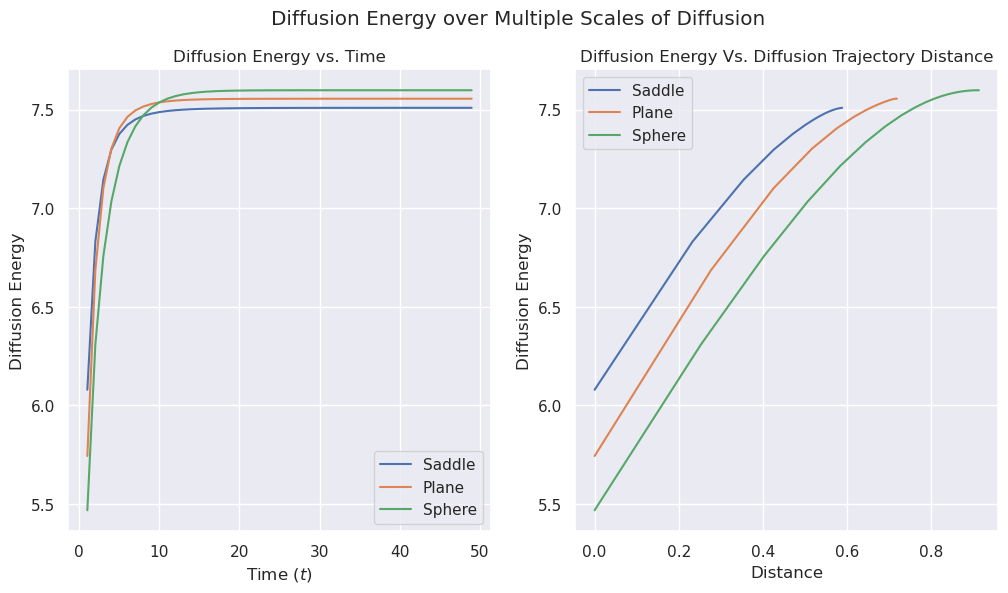
\includegraphics{index_files/figure-latex/fig-curvature-curves-output-2.png}

}

\caption{\label{fig-curvature-curves}Diffusion energies across multiple
scales on a 4-dimensional saddle, plane, and sphere (all 3-manifolds).
When comparing directly between times, there is no clear separation of
curvatures. Aligning diffusions by diffusion trajectory distance reveals
curvature. Source:
\href{https://professorwug.github.io/diffusion-curvature//Users/adjourner/Pumberton/Workshop/21-SUMRY-Curvature/diffusion-curvature/nbs/3d-diffusion-trajectory-distance-normalization.ipynb.html\#cell-fig-curvature-curves}{Standard
libraries}}

\end{figure}

Applying diffusion trajectory alignment to our diffusion energies also
has the happy effect of focusing our measurement on the most relevant
scales of diffusion. When using diffusion times, one must be careful to
select a time around the `elbow' of the diffusion energies
(Definition~\ref{def-energy-of-diffusion}). Smaller \(T\)'s yield more
localized measurements of curvature. But make \(t\) too small, and the
diffusion might have barely differentiated itself from a dirac, drowning
the curvature in sampling-induced noise. Yet make \(t\) too large, and
the diffusion will progress to the uninformative steady-state
distribution. With the diffusion trajectory distance, all of the
undesirably large \(t\)'s are compressed into a narrow range of
distances -- the diffusion trajectory limits to the steady state
distribution, and the diffusion trajectory distances that correspond to
it are all within some \(\epsilon\) of the maximum diffusion trajectory
distance. Finding a time around the elbow of the diffusion energies then
corresponds to choosing a diffusion distance within \(80-95\)\% of the
maximum; and via the inverse diffusion trajectory distance, \(t_{DTD}\),
this can be translated to the appropriate scale of \(t\) for each
dataset.

In practice, we don't have access to a metric \(g_{p}\) on the
probability simplex; this space is too high-dimensional, and we lack a
continuous parameterization of graph diffusion. Instead, we approximate
this integral by measuring the distances between subsequent diffusions
(performed for every integer \(1 \leq t \leq T(d)\)). This approximates
the diffusion trajectory distances for each scale of diffusion, giving
us discrete examples of \(d_{DTD}\). We then construct a piecewise
linear approximation of \(d_{DTD}\) to estimate the inverse,
\(t_{DTD}\).

\subsubsection{The Curvature-Agnostic Kernel \& Automatic Bandwidth
Tuning}\label{the-curvature-agnostic-kernel-automatic-bandwidth-tuning}

Diffusion trajectory alignment significantly reduces the interference
caused by graph construction, but does not completely eliminate it. Due
to our lack of access to a diffusion coordinate space metric, and the
approximations used for the diffusion trajectory distance, we find the
robustness of our algorithm is significantly improved by a few
adjustments to standard graph construction techniques to make them more
curvature agnostic.

To turn a point cloud into a graph, one places a kernel (e.g.~a
gaussian) at each point, and assigns edges to surrounding points with
weights given by the kernel. The main parameter here is the bandwidth of
each kernel: make it too high, and everything is connected; too low, and
points are isolated. Moreover, the distances between a point and its
neighbors may vary. Where the points are sparse, one wants a higher
bandwidth. Where dense, a lower bandwidth.

A standard technique for accommodating the variable densities of point
cloud data is a \(k\)-neighbor \emph{adaptive kernel}. Here, the
bandwidth at each point is set to the squared distance to the \(k\)-th
nearest neighbor, averaged in some way between the two inputs. Here's
one standard adaptive kernel:

\[
\begin{aligned}
k(x, y) & =\frac{e^{-\frac{d(x, y)^2}{d(x, N_{k}(x))^2}}}{d(y, N_{k}(y))}
+\frac{e^{-\frac{d(x, y)^2}{d(y, N_{k}(x))^2}}}{d(x, N_{k}(y)}
\end{aligned}
\]

where \(N_{k}(x)\) gives the \(k\)th nearest neighbor to \(x\).

Note that that parameter \(k\) plays roles in two kinds of adaptation.
By setting the bandwidth to some Euclidean distance \(d(x,N_{k}(x))\)
between data points, it adapts the kernel to the \emph{right scale} for
the point cloud, concentrating its probability within a local
neighborhood. It also controls the \emph{size} of that local
neighborhood; typically set between 5 and 15.

Unfortunately, this adaptive process hinges on the correspondence
between the Euclidean distances \(d(x,N_{k}(x))\), and the manifold
distances -- a correspondence that degrades \emph{faster} the higher the
magnitude of curvature! Consider a highly-curved paraboloid. The
Euclidean distance from its center point to its nearest few neighbors is
roughly the geodesic distance. But as the neighborhood widens, and the
neighbors move higher up the paraboloid, the Euclidean distance now
underestimates the true geodesic distance: it cuts across the manifold.
This happens in spaces of high positive or high negative curvature.

As a result, the adaptive kernel constructed in highly curved spaces has
a smaller bandwidth than in flat spaces, even using the same kernel
parameters. If one directly compares the laziness of diffusion on two
such graphs, it will appear lazier than on the flat manifold.

To remedy this, we make a simple adjustment to the standard adaptive
kernel. The key is separating the parameter which controls neighborhood
size from neighborhood scale. In the adaptive kernel, both are
controlled by the parameter \(k\); as discussed above, in spaces of high
curvature, the same \(k\) creates different scales. Instead, we always
set \(k = 1\) and use another parameter -- \(\nu\), the neighbor-size --
to control the variance of the kernel.

\[
\begin{aligned}
k(x, y) & =\frac{e^{-\frac{d(x, y)^2}{d(x, N_{k}(x))^2\nu^2}}}{d(y, N_{k}(y))}
+\frac{e^{-\frac{d(x, y)^2}{d(y, N_{k}(x))^2\nu^2}}}{d(x, N_{k}(y)}
\end{aligned}
\]

\(\nu\) behaves like the kernel bandwidth in the regular fixed Gaussian
kernel. We call this the \emph{Curvature-Agnostic Kernel}.

\begin{itemize}
\tightlist
\item[$\square$]
  Figure comparing the adaptive to curvature agnostic kernels with
  diffusion trajectory normalization. Use a stacked image.
\end{itemize}

Figure WAWA illustrates the increased robustness diffusion trajectory
alignment gains from using this curvature-agnostic kernel. The relative
ordering of graphs is still achieved by the traditional adaptive kernel,
but is significantly denoised by these tweaks.

The main parameter of the curvature-agnostic kernel is the ``neighbor
scale'' \(\nu\), which sets the kernel bandwidth to the specified
multiple of the average distance to the \(k\)th-nearest neighbor. As a
single parameter, this can be tuned easily. We use as a heuristic the
desired median number of points with non-negligible single-step
diffusion probability, and perform a binary search over values of
\(\nu\) until this number is within a desired tolerance.

We suspect the curvature-agnostic kernel may be generally useful in
manifold learning. In any downstream analysis that leverages the graph
geometry -- be it distance estimation, {[}CITE HUGUET{]} or metric
learning {[}CITE US{]} -- this analysis is made easier by a kernel whose
bandwidth does not gratuitously fluctuate in regions of high curvature.

\begin{itemize}
\tightlist
\item[$\square$]
  Can we provide experimental results here? Does PHATE or HeatGeo
  perform better with this kernel?
\end{itemize}

\section{The Curvature Colosseum: A Discrete Curvature Benchmarking
Suite}\label{the-curvature-colosseum-a-discrete-curvature-benchmarking-suite}

The discrete curvature literature lacks a standard benchmark. Previous
work has used a combination of evaluations on 2-dimensional toy
manifolds (where correctness is visually obvious) and generally one or
two bespoke higher-dimensional test cases, on which the target method is
extensively tuned -- and even then, often has ambiguous results.
Comparisons between methods have been scarce.

Thus, Ollivier-Ricci curvature was introduced mostly on toy-examples. It
has since been compared to Forman-Ricci (BASTIAN) ??? Hickok \& Blumberg
primarily tested their method on the 2-dimensional torus and sphere.
They compared to WAWA. However, their point clouds weren't uniformly
sampled with respect to the manifold geometry - causing some density
artifacts. CHECK! Sritharan et al.~performed the most extensive testing
we have seen, with studies of correlation against ground truth and
robustness to parameters. Zhang et al.~compared accuracy at a variety of
noise scales to Hickok \& Blumberg and to our previous unsigned
diffusion laziness curvature, but only on 2-dimensional manifolds.

To overcome these shortcomings, we propose a discrete-curvature
benchmarking suite we affectionately dub the `Curvature Colosseum.' It
permits standardized comparison between methods on three axes:

\begin{enumerate}
\def\labelenumi{\arabic{enumi}.}
\tightlist
\item
  \emph{Resilience to Noise.} Pearson correlations with ground truth
  curvature on 2-Dimensional manifolds across noise scales.
\item
  \emph{Accuracy on High Dimensions.} Pearson correlations with ground
  truth curvature on 3-8 dimensional surfaces.
\item
  \emph{Sign Prediction}. Ability to distinguish spaces of positive,
  negative, and zero curvature in dimensions 3-8.
\end{enumerate}

Each of the manifolds used above is rejection sampled (CITE SOMEONE) to
ensure uniform density with respect to manifold volume. When
benchmarking curvature methods from the literature, we use their
suggested parameters when available.

We provide full implementation details in the appendix. Our code is
available at GITHUB LINK, along with a public dashboard of the results
at ANOTHER LINK.

The remaining parts of this section detail the results of Diffusion
Curvature and its competition on each axis of the Colosseum.

\subsection{Performance in Low Dimensions under
Noise}\label{performance-in-low-dimensions-under-noise}

\begin{figure}[H]

{\centering 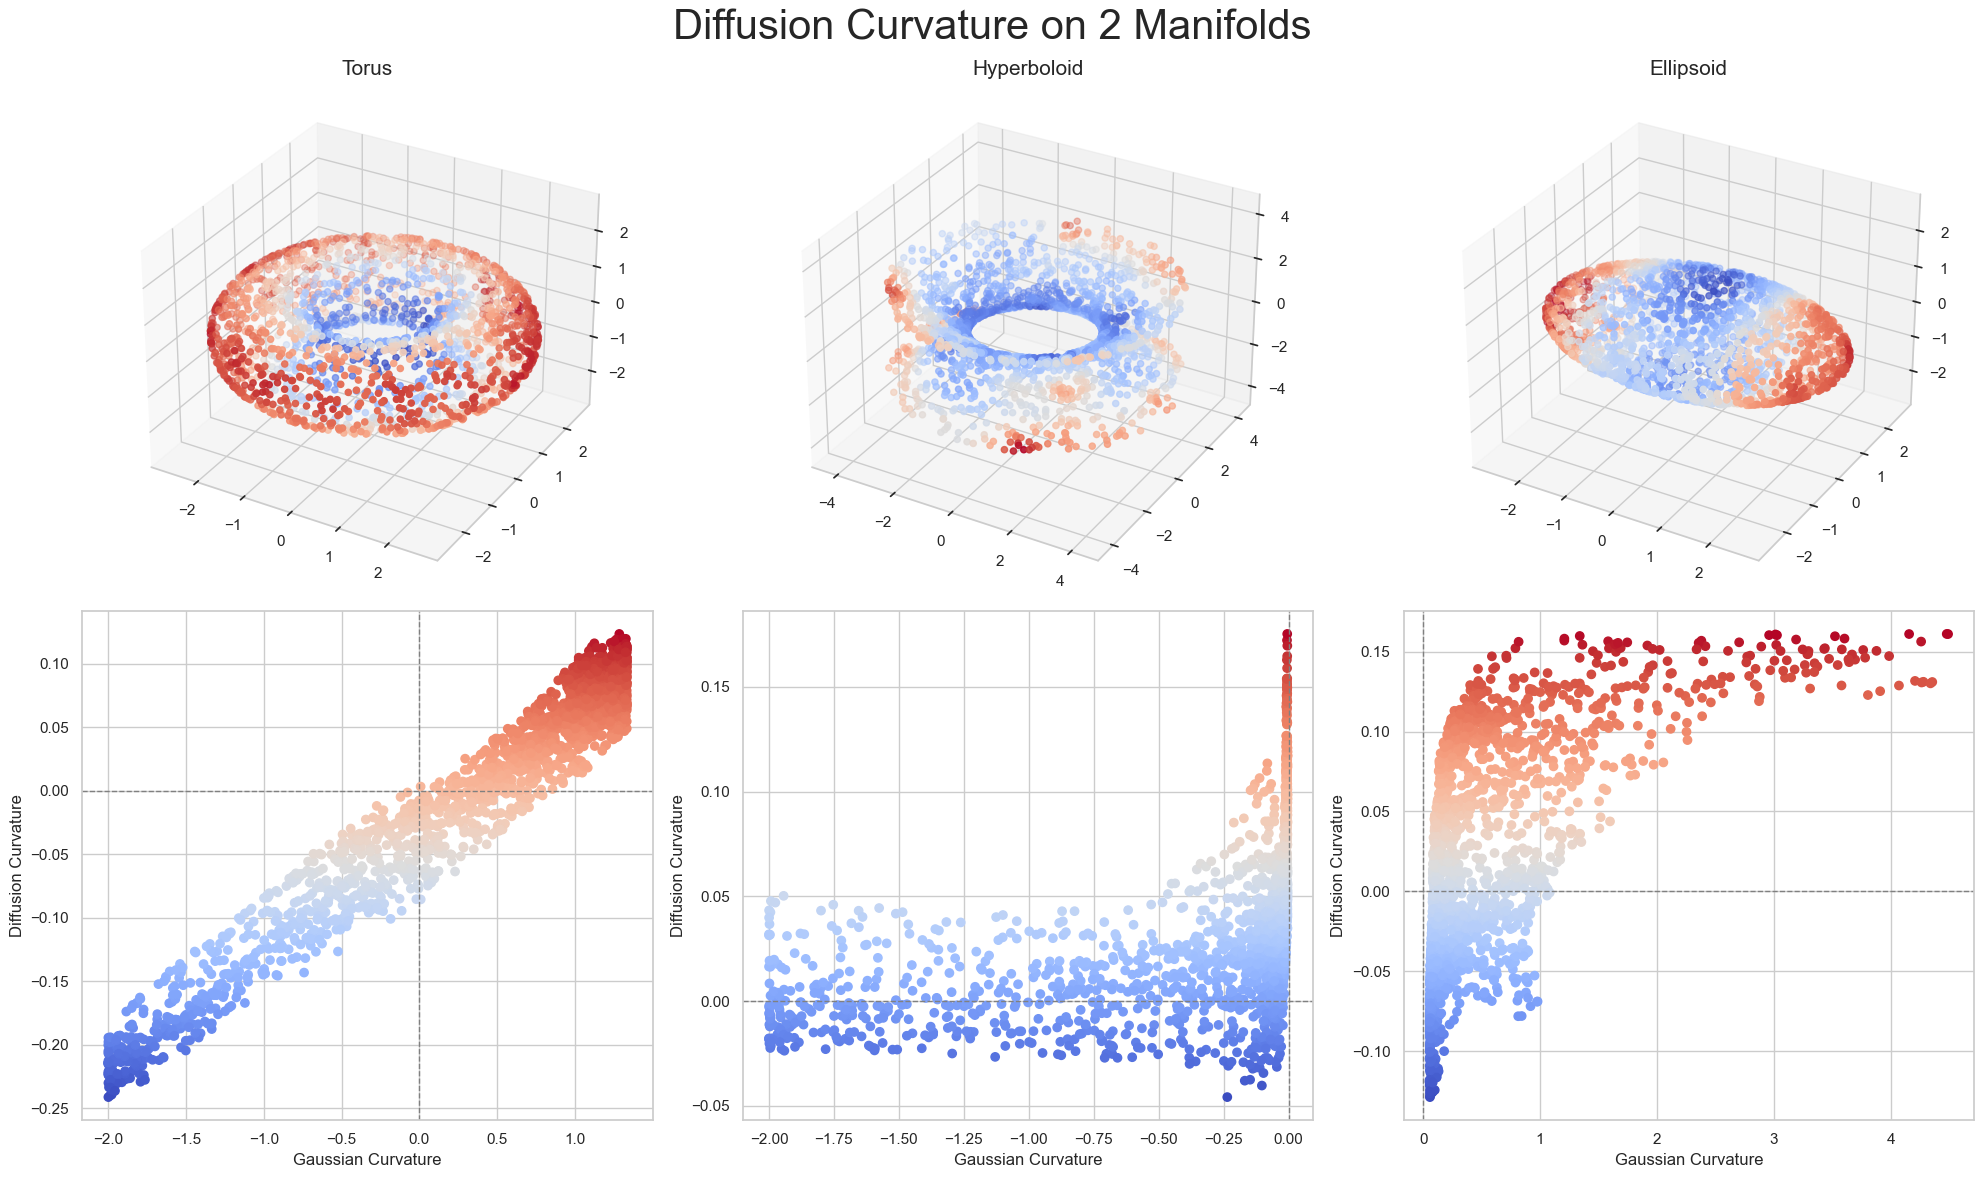
\includegraphics{index_files/figure-latex/fig-2-manifolds-output-1.png}

}

\caption{\label{fig-2-manifolds}Diffusion Curvature vs Gaussian
Curvature on 2-Manifolds. Source:
\href{https://professorwug.github.io/diffusion-curvature//Users/adjourner/Pumberton/Workshop/21-SUMRY-Curvature/diffusion-curvature/nbs/2a-Diffusion-Curvatures-of-Toy-Manifolds.ipynb.html\#cell-fig-2-manifolds}{Standard
libraries}}

\end{figure}

First, a sanity check. Does diffusion curvature recover the Gaussian
curvature of basic 2-manifolds? Figure~\ref{fig-2-manifolds} shows the
diffusion curvature of a Torus, Hyperboloid, and Ellipsoid, along with a
scatter plot correlating diffusion curvature and Gaussian curvature.
Figure~\ref{fig-2-manifolds-visual-comparison} places this in the
context of existing methods.

\begin{figure}[H]

{\centering 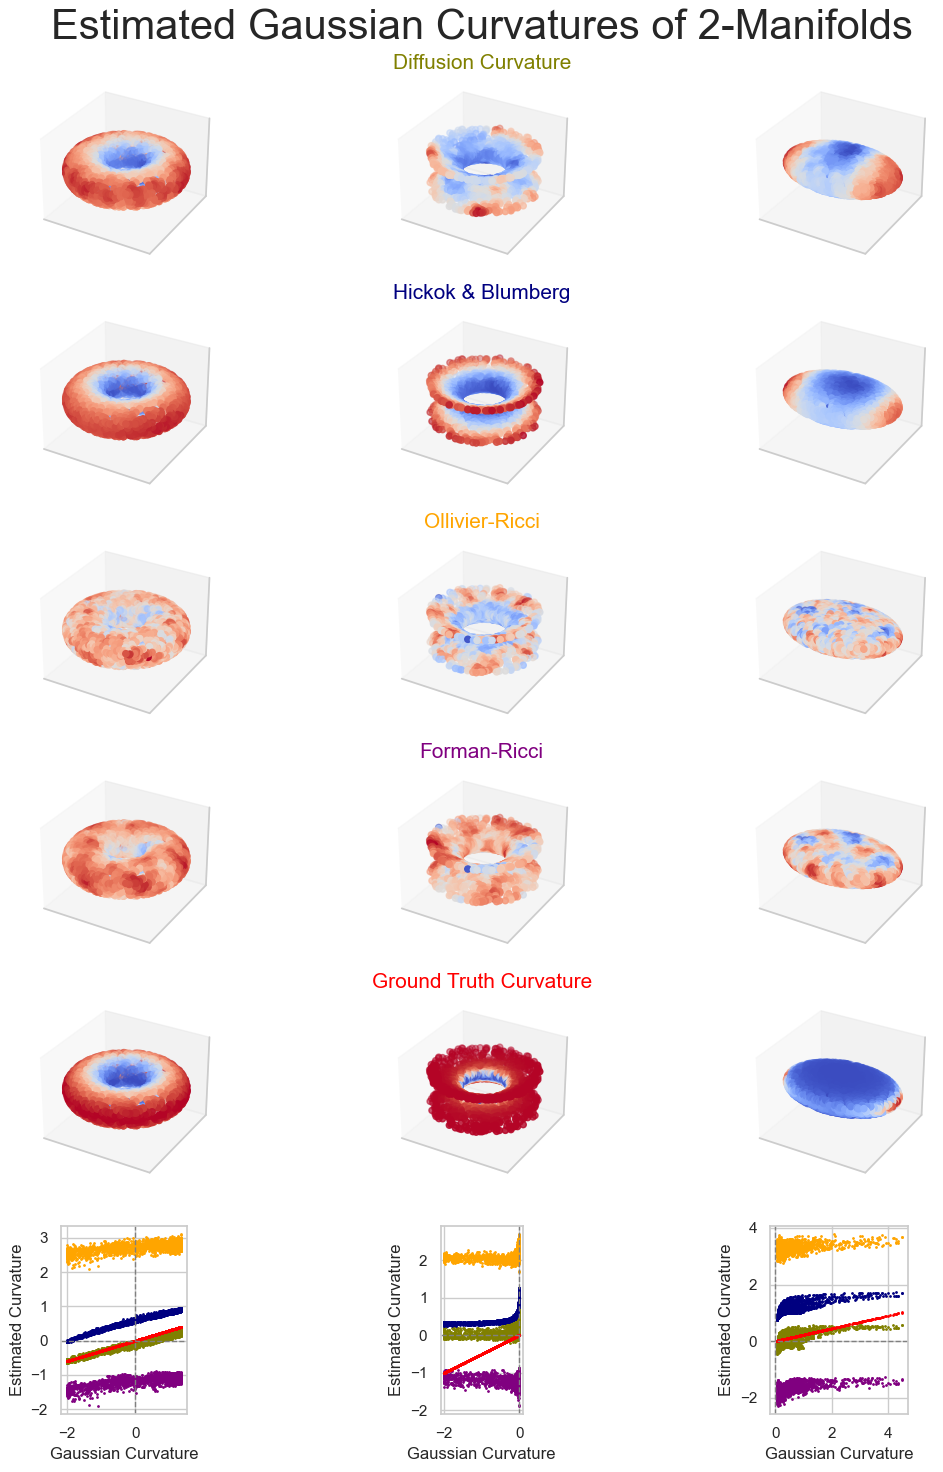
\includegraphics{index_files/figure-latex/fig-2-manifolds-visual-comparison-output-1.png}

}

\caption{\label{fig-2-manifolds-visual-comparison}Diffusion Curvature vs
Gaussian Curvature on 2-Manifolds. Source:
\href{https://professorwug.github.io/diffusion-curvature//Users/adjourner/Pumberton/Workshop/21-SUMRY-Curvature/diffusion-curvature/nbs/2-Toy-Manifolds-Benchmark.ipynb.html\#cell-fig-2-manifolds-visual-comparison}{Standard
libraries}}

\end{figure}

All of these methods in Figure~\ref{fig-2-manifolds-visual-comparison}
approximately give the correct relative coloring of these 2-manifolds,
except perhaps Forman-Rici. As expected, the graph-based methods,
Ollivier-Ricci and Forman-Ricci, perform the worst; they weren't
designed to deal with the noise of pointcloud data. Hickok \& Blumberg's
definition performs the best in terms of correspondence with the ground
truth Gaussian curvature, but diffusion curvature follows it closely.
Observing the bottom panel of
Figure~\ref{fig-2-manifolds-visual-comparison}, we can see diffusion
curvature corresponding closely with the red line of ground truth
curvature.

In Table Figure~\ref{fig-2-manifolds-noise-table}, we see the results of
adding Gaussian noise to each manifold. Here, the noise resilience of
diffusion geometry grants diffusion curvature a huge advantage. It has
the highest pearson correlation with the ground truth under all but the
smallest scales of noise for the torus and ellipsoid. We suspect its
correlation with the hyperboloid is lower than Hickok \& Blumberg's only
because of the ``edge'' of this negatively-curved manifold, which
creates the appearance of positive curvature.

\begin{figure}

{\centering 

\begin{longtable}[]{@{}lllllllllllllllllll@{}}
\toprule\noalign{}
\multicolumn{19}{@{}l@{}}{%
Curvature on 2-Manifolds with Noise} \\
\multicolumn{19}{@{}l@{}}{%
Pearson correlations and sign accuracies} \\
\midrule\noalign{}
\endhead
\bottomrule\noalign{}
\endlastfoot
\multirow{2}{*}{Model \& Metric} & \multicolumn{6}{l}{%
{Torus}} & \multicolumn{6}{l}{%
{Hyperboloid}} & \multicolumn{6}{l@{}}{%
{Ellipsoid}} \\
& Torus & Torus noise = 0.05 & Torus noise = 0.1 & Torus noise = 0.15 &
Torus noise = 0.2 & Torus noise = 0.25 & Hyperboloid & Hyperboloid noise
= 0.05 & Hyperboloid noise = 0.1 & Hyperboloid noise = 0.15 &
Hyperboloid noise = 0.2 & Hyperboloid noise = 0.25 & Ellipsoid &
Ellipsoid noise = 0.05 & Ellipsoid noise = 0.1 & Ellipsoid noise = 0.15
& Ellipsoid noise = 0.2 & Ellipsoid noise = 0.25 \\
\multicolumn{19}{@{}l@{}}{%
Pearson Correlation} \\
Diffusion Curvature & 0.979 & 0.978 & 0.978 & 0.972 & 0.959 & 0.937 &
0.471 & 0.501 & 0.475 & 0.422 & 0.350 & 0.297 & 0.606 & 0.626 & 0.638 &
0.640 & 0.634 & 0.621 \\
Forman-Ricci & 0.717 & 0.734 & 0.764 & 0.768 & 0.765 & 0.771 & −0.106 &
−0.090 & −0.080 & −0.094 & −0.150 & −0.198 & 0.482 & 0.511 & 0.522 &
0.509 & 0.507 & 0.502 \\
Hickok \& Blumberg & 0.987 & 0.978 & 0.950 & 0.910 & 0.861 & 0.811 &
0.651 & 0.650 & 0.644 & 0.634 & 0.622 & 0.614 & 0.734 & 0.745 & 0.704 &
0.623 & 0.544 & 0.479 \\
Ollivier-Ricci & 0.614 & 0.625 & 0.664 & 0.685 & 0.699 & 0.704 & 0.389 &
0.375 & 0.367 & 0.347 & 0.328 & 0.324 & 0.359 & 0.369 & 0.380 & 0.394 &
0.410 & 0.407 \\
\multicolumn{19}{@{}l@{}}{%
Sign Accuracy} \\
Diffusion Curvature & 0.903 & 0.849 & 0.341 & 0.341 & 0.916 & 0.341 &
0.190 & 0.000 & 0.266 & 0.235 & 0.000 & 1.000 & 0.509 & 0.529 & 0.251 &
0.000 & 0.000 & 0.000 \\
Forman-Ricci & 0.341 & 0.341 & 0.341 & 0.341 & 0.341 & 0.341 & 1.000 &
1.000 & 1.000 & 1.000 & 1.000 & 1.000 & 0.000 & 0.000 & 0.000 & 0.000 &
0.000 & 0.000 \\
Hickok \& Blumberg & 0.696 & 0.810 & 0.878 & 0.406 & 0.365 & 0.365 &
0.000 & 0.000 & 0.215 & 0.415 & 0.474 & 0.501 & 1.000 & 1.000 & 0.098 &
0.002 & 0.002 & 0.002 \\
Ollivier-Ricci & 0.659 & 0.659 & 0.659 & 0.659 & 0.659 & 0.659 & 0.000 &
0.000 & 0.000 & 0.000 & 0.000 & 0.000 & 1.000 & 1.000 & 1.000 & 1.000 &
1.000 & 1.000 \\
\end{longtable}

}

\caption{\label{fig-2-manifolds-noise-table}Performance of methods under
noise on 2-Manifolds with Noise. Source:
\href{https://professorwug.github.io/diffusion-curvature//Users/adjourner/Pumberton/Workshop/21-SUMRY-Curvature/diffusion-curvature/nbs/2-Toy-Manifolds-Benchmark.ipynb.html\#cell-fig-2-manifolds-noise-table}{Standard
libraries}}

\end{figure}

\subsection{Performance in High Dimensions under
Noise}\label{performance-in-high-dimensions-under-noise}

TBD!

\subsection{Sign Differentiation}\label{sign-differentiation}

To test the ability to differentiate negative from positive curvature in
high dimensions, we constructed a dataset containing saddle points,
planes, and spheres in dimensions 2-6. For planes, we used uniform
samples from the \(d\)-dimensional unit cube; for spheres, we sampled
points from a Gaussian in \(\mathbb{R}^d\) and normalized them to have
unit length; for saddles, we constructed a quadric surface with the sign
of each quadratic alternating between dimensions, and performed
rejection sampling on the resulting parameterization. We sampled 2000
points from each surface, and performed this sampling 20 times per
surface, creating a dataset of 60 point clouds of negative, zero, and
positive curvature.

To make the comparison as fair as possible, we use our
curvature-agnostic kernel to construct the graphs used for Forman-Ricci
and Ollivier-Ricci curvature instead of the standard adaptive or
k-nearest neighbor kernels generally used (which give worse
performance). Hickok \& Bloomberg's definition operates directly on
pointclouds, so we leave it as is.

As seen in Figure~\ref{fig-sadspheres}, only diffusion curvature
differentiates the sign across all dimensions. Hickok \& Blumberg's
curvature initially correctly classifies saddles as negatively curved
and spheres as positive in dimension 2, however in dimensions 3-5, it
classifies everything as negatively curved, with planes given a higher
negative curvature than saddles. By dimension 6, it assigns the most
negatively curved surface the least degree of negative curvature. For
Ollivier-Ricci, the variance within samplings is extremely high (an
artifact of applying a graph-based definition to noisy pointclouds), but
it both describes all curvatures as positive and gives the
negatively-curved dataset the highest positive curvature. Forman-Ricci
does the best among these, comparatively; it at least gives saddles,
spheres, and planes the correct ordering of curvature. However the
magnitude of its curvatures is entirely negative; there's no sign
differentiation.

Diffusion curvature both preserves the correct relative ordering and
distinguishses between the signs of saddles and spheres with 95\%
accuracy.

\begin{figure}[H]

{\centering 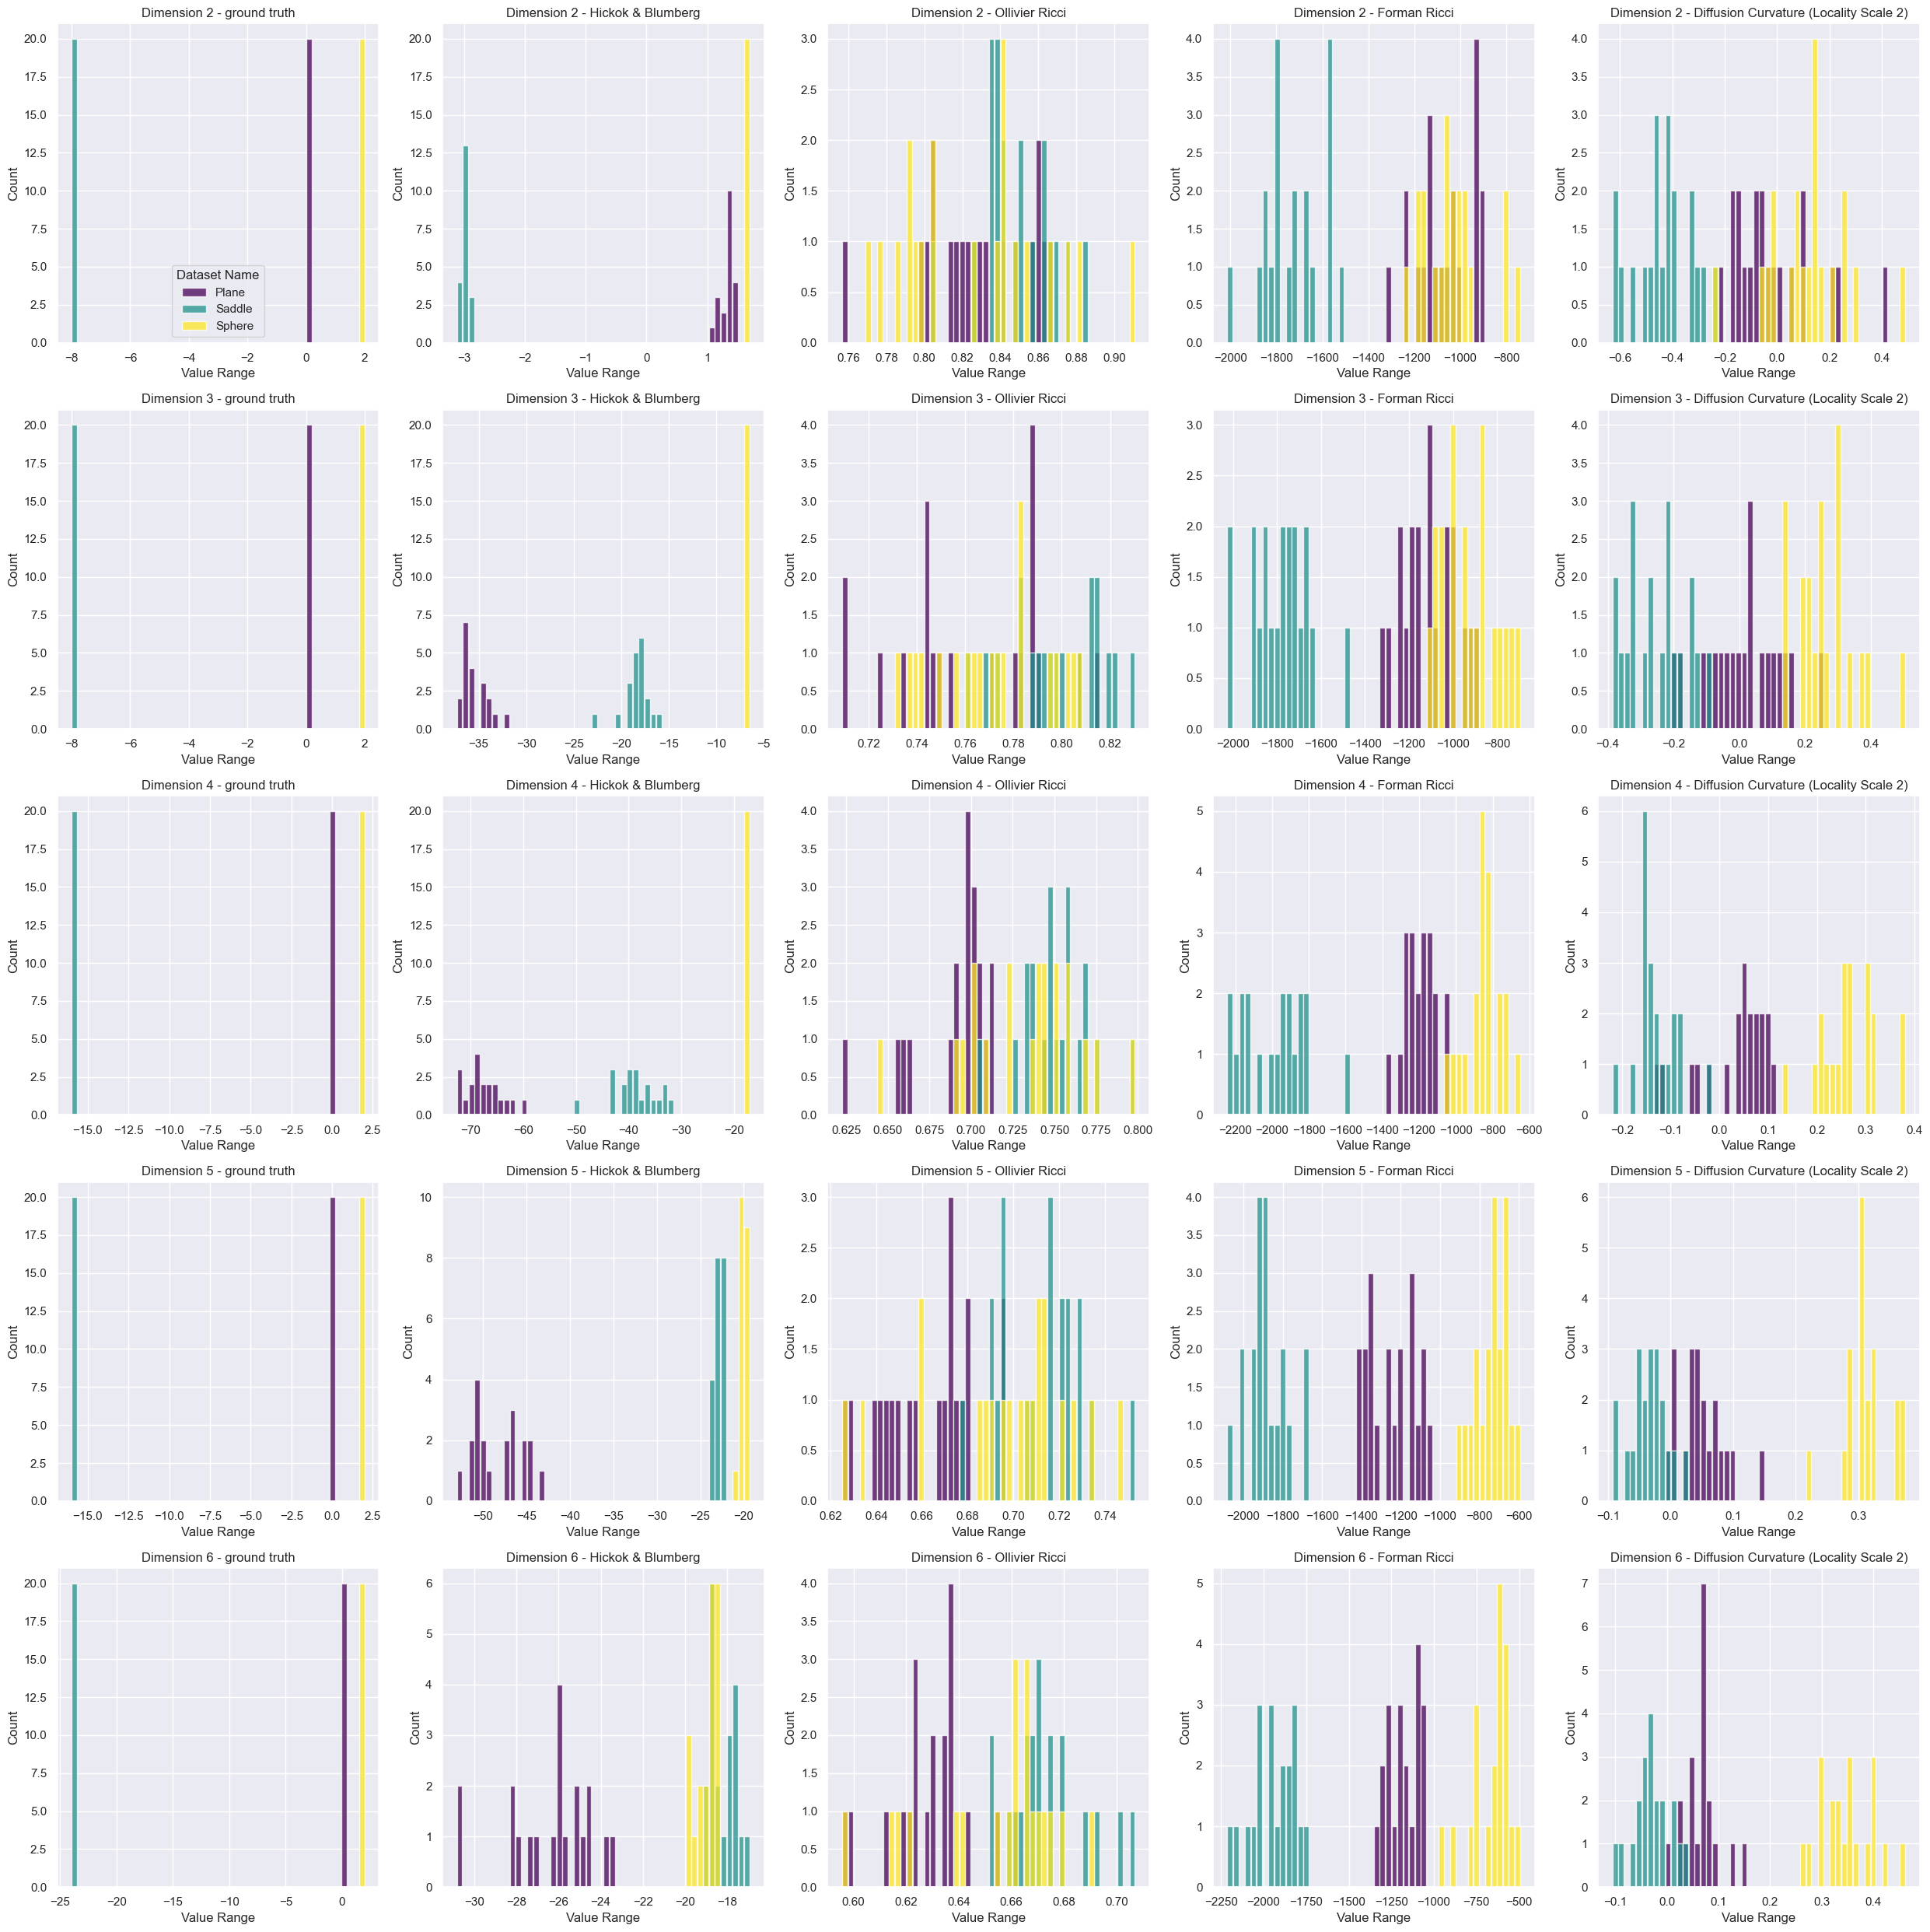
\includegraphics{index_files/figure-latex/fig-sadspheres-output-1.png}

}

\caption{\label{fig-sadspheres}Predicted curvatures of Saddles and
Spheres in dimensions 2-6. Diffusion Curvature robustly distinguishes
between the signs of the data, even in high dimensions, and with
relative sparsity. Source:
\href{https://professorwug.github.io/diffusion-curvature//Users/adjourner/Pumberton/Workshop/21-SUMRY-Curvature/diffusion-curvature/nbs/5-sign-prediction-tests.ipynb.html\#cell-fig-sadspheres}{Standard
libraries}}

\end{figure}

\subsection{Resilience to Parameters}\label{resilience-to-parameters}

\section{Applications}\label{applications}

\subsection{Loss Landscapes}\label{loss-landscapes}

\subsection{Curvature as a TDA
Filtration}\label{curvature-as-a-tda-filtration}

\section{Related Work}\label{related-work}

\subsection{Foreman Ricci Curvature}\label{foreman-ricci-curvature}

\subsection{Hickock \& Blumberg's Volume Comparison
Curvature}\label{hickock-blumbergs-volume-comparison-curvature}

\subsection{Sritharan}\label{sritharan}

\section{Conclusion}\label{conclusion}

\section*{References}\label{references}
\addcontentsline{toc}{section}{References}

\phantomsection\label{refs}
\setlength{\cslentryspacing}{0em}
\begin{CSLReferences}
\bibitem[\citeproctext]{ref-bhaskar2022DiffusionCurvatureEstimating}
Bhaskar, Dhananjay, Kincaid MacDonald, Oluwadamilola Fasina, Dawson
Thomas, Bastian Rieck, Ian Adelstein, and Smita Krishnaswamy. 2022.
{``Diffusion Curvature for Estimating Local Curvature in High
Dimensional Data.''} \emph{Advances in Neural Information Processing
Systems} 35: 21738--49.
\url{https://proceedings.neurips.cc/paper_files/paper/2022/hash/88438dc62fc5c8777e2b5f1b4f6d37a2-Abstract-Conference.html}.

\bibitem[\citeproctext]{ref-2021BishopGromovInequality}
{``Bishop--{Gromov} Inequality.''} 2021. In \emph{Wikipedia}.
\url{https://en.wikipedia.org/w/index.php?title=Bishop\%E2\%80\%93Gromov_inequality&oldid=1059331416}.

\bibitem[\citeproctext]{ref-coifman2006DiffusionMaps}
Coifman, Ronald R., and Stéphane Lafon. 2006. {``Diffusion Maps.''}
\emph{Applied and Computational Harmonic Analysis}, Special {Issue}:
{Diffusion Maps} and {Wavelets}, 21 (1): 5--30.
\url{https://doi.org/10.1016/j.acha.2006.04.006}.

\bibitem[\citeproctext]{ref-fasina2023NeuralFIMLearning}
Fasina, Oluwadamilola, Guillaume Huguet, Alexander Tong, Yanlei Zhang,
Guy Wolf, Maximilian Nickel, Ian Adelstein, and Smita Krishnaswamy.
2023. {``Neural {FIM} for Learning {Fisher Information Metrics} from
Point Cloud Data.''} June 11, 2023.
\url{https://doi.org/10.48550/arXiv.2306.06062}.

\bibitem[\citeproctext]{ref-hickok2023IntrinsicApproachScalarCurvature}
Hickok, Abigail, and Andrew J. Blumberg. 2023. {``An {Intrinsic
Approach} to {Scalar-Curvature Estimation} for {Point Clouds}.''} arXiv.
\url{https://doi.org/10.48550/arXiv.2308.02615}.

\bibitem[\citeproctext]{ref-huguet2023HeatDiffusionPerspective}
Huguet, Guillaume, Alexander Tong, Edward De Brouwer, Yanlei Zhang, Guy
Wolf, Ian Adelstein, and Smita Krishnaswamy. 2023. {``A {Heat Diffusion
Perspective} on {Geodesic Preserving Dimensionality Reduction}.''} May
30, 2023. \url{https://doi.org/10.48550/arXiv.2305.19043}.

\bibitem[\citeproctext]{ref-moon2019VisualizingStructureTransitions}
Moon, Kevin R., David van Dijk, Zheng Wang, Scott Gigante, Daniel B.
Burkhardt, William S. Chen, Kristina Yim, et al. 2019. {``Visualizing
Structure and Transitions in High-Dimensional Biological Data.''}
\emph{Nature Biotechnology} 37 (12, 12): 1482--92.
\url{https://doi.org/10.1038/s41587-019-0336-3}.

\bibitem[\citeproctext]{ref-ollivier2009RicciCurvatureMarkov}
Ollivier, Yann. 2009. {``Ricci Curvature of {Markov} Chains on Metric
Spaces.''} \emph{Journal of Functional Analysis} 256 (3): 810--64.
\url{https://doi.org/10.1016/j.jfa.2008.11.001}.

\bibitem[\citeproctext]{ref-saloff-coste2010HeatKernelIts}
Saloff-Coste, Laurent. 2010. {``The Heat Kernel and Its Estimates.''} In
\emph{Advanced {Studies} in {Pure Mathematics}}, 405--36. Kyoto
University, Japan. \url{https://doi.org/10.2969/aspm/05710405}.

\bibitem[\citeproctext]{ref-tong2021DiffusionEarthMovera}
Tong, Alexander Y., Guillaume Huguet, Amine Natik, Kincaid Macdonald,
Manik Kuchroo, Ronald Coifman, Guy Wolf, and Smita Krishnaswamy. 2021.
{``Diffusion {Earth Mover}'s {Distance} and {Distribution
Embeddings}.''} In \emph{Proceedings of the 38th {International
Conference} on {Machine Learning}}, 10336--46. PMLR.
\url{https://proceedings.mlr.press/v139/tong21a.html}.

\bibitem[\citeproctext]{ref-tong2021DatadrivenLearningGeometric}
Tong, Alexander, Frederick Wenkel, Kincaid Macdonald, Smita
Krishnaswamy, and Guy Wolf. 2021. {``Data-Driven Learning of Geometric
Scattering Modules for Gnns.''} In \emph{2021 {IEEE} 31st {International
Workshop} on {Machine Learning} for {Signal Processing} ({MLSP})}, 1--6.
IEEE. \url{https://ieeexplore.ieee.org/abstract/document/9596169/}.

\end{CSLReferences}



\end{document}
